\section{Background} \label{sec-background}
In this section, we first provide the workflow of a collaborative data science platform, which we use throughout the paper and outline the challenges and inefficiencies of the platform.
Next, we describe experiment databases and how they can improve the execution of machine learning workloads.

\subsection{Motivating Example}\label{subsec-motivational-example}
Kaggle is a data science competition platform which enables organizations to host data science challenges.
Users participate in the challenges, write solutions, and submit these solutions to the platform.
To arrive at their final solutions, participants utilize the infrastructure provided by Kaggle to write data analysis and machine learning workloads either in the form of R and Python scripts \hladd{(a long running workload)} or Jupyter notebooks \hladd{(interactive workloads)} and execute them on the Kaggle's platform.
Users can also make their workloads publicly available to other users.
As a result, many Kaggle users work together to find high-quality solutions.

Kaggle utilizes docker containers to provide isolated computational environments called Kaggle kernels.
Kaggle groups kernels by competition. Figure \ref{example-use-case} shows the infrastructure of Kaggle.
Each kernel has limited CPU, GPU, disk space, and memory (i.e., 4 CPU cores, 17 GB of RAM, 5 GB of disk space, and a maximum of 9 hours of execution time. GPU kernels have 2 CPU cores and 13 GB of RAM\footnote{https://www.kaggle.com/docs/kernels}).
In busy times, this results in users to be placed in queues (especially for GPU-enabled machines) until resources become available.

\begin{figure}
\centering
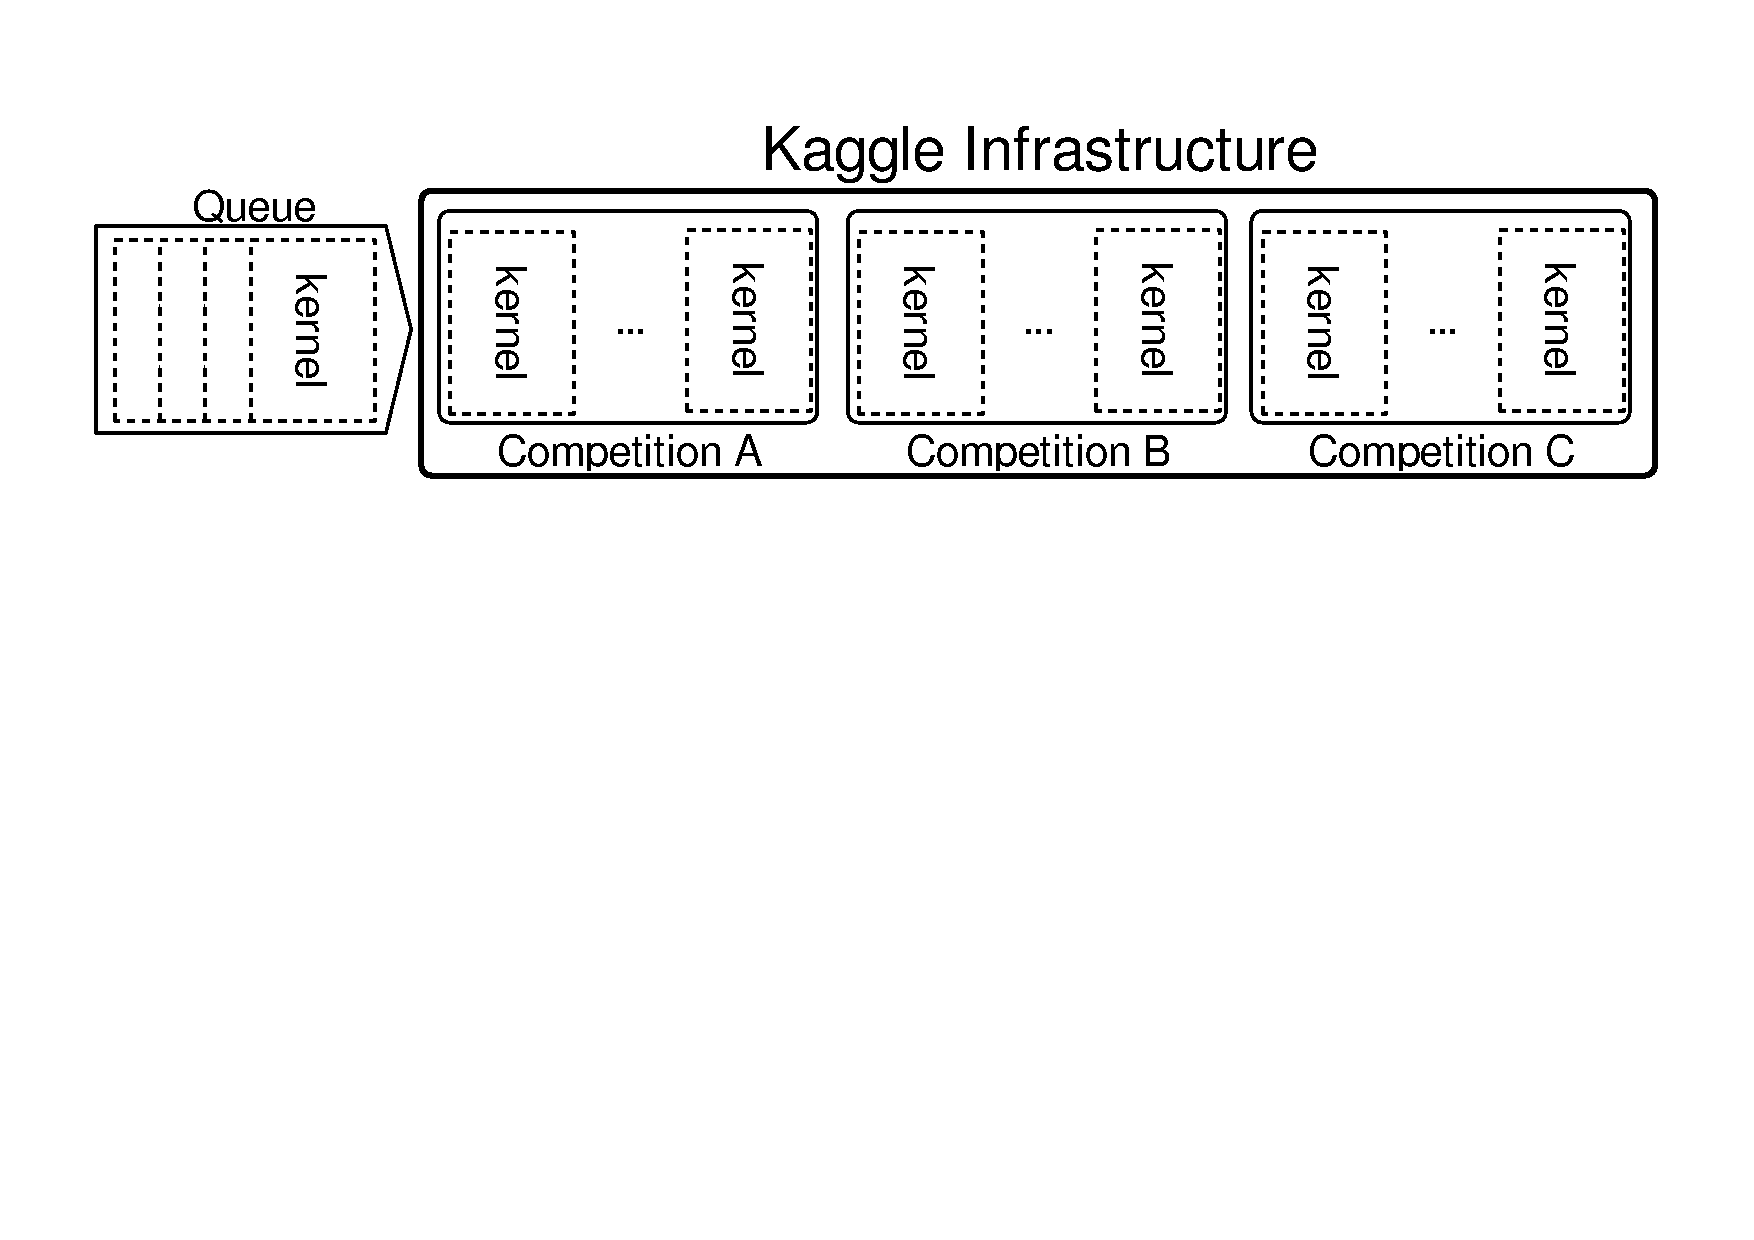
\includegraphics[width=\columnwidth]{../images/example-use-case}
\caption{Kaggle Infrastructure}
\label{example-use-case}
\end{figure}

Every user who participates in a Kaggle competition has the same goal, which is to solve the task described by the competition organizer.
Typically, the task is to design a machine learning workload containing a series of exploratory data analysis steps to preprocess one or multiple raw datasets provided by the competition organizer, followed by a model training step to train a machine learning model, which aims to maximize a quality metric on an evaluation dataset.
For example, in the \textit{Titanic: Machine Learning from Disaster} competition in Kaggle\footnote{https://www.kaggle.com/c/titanic}, the task is to create a machine learning pipeline and train a classification model on the Titanic training dataset that can predict if a traveler survived the Titanic disaster, with the goal of maximizing the prediction accuracy on a separate test dataset.
When solving the same tasks, users tend to utilize the same type of operations.
Figure \ref{fig-titanic-script-hierarchy} shows the most popular kernels and \hl{their relationship} for the Titanic competition.
% Tilmann: seems that this is something you define? how does this help your analysis? Behrouz: I'm trying to motivate the fact that people implicitly or explicitly use similar operations. Here, 'relationship' mean when an author explicitly cites another work in his script.
\begin{figure}
\centering
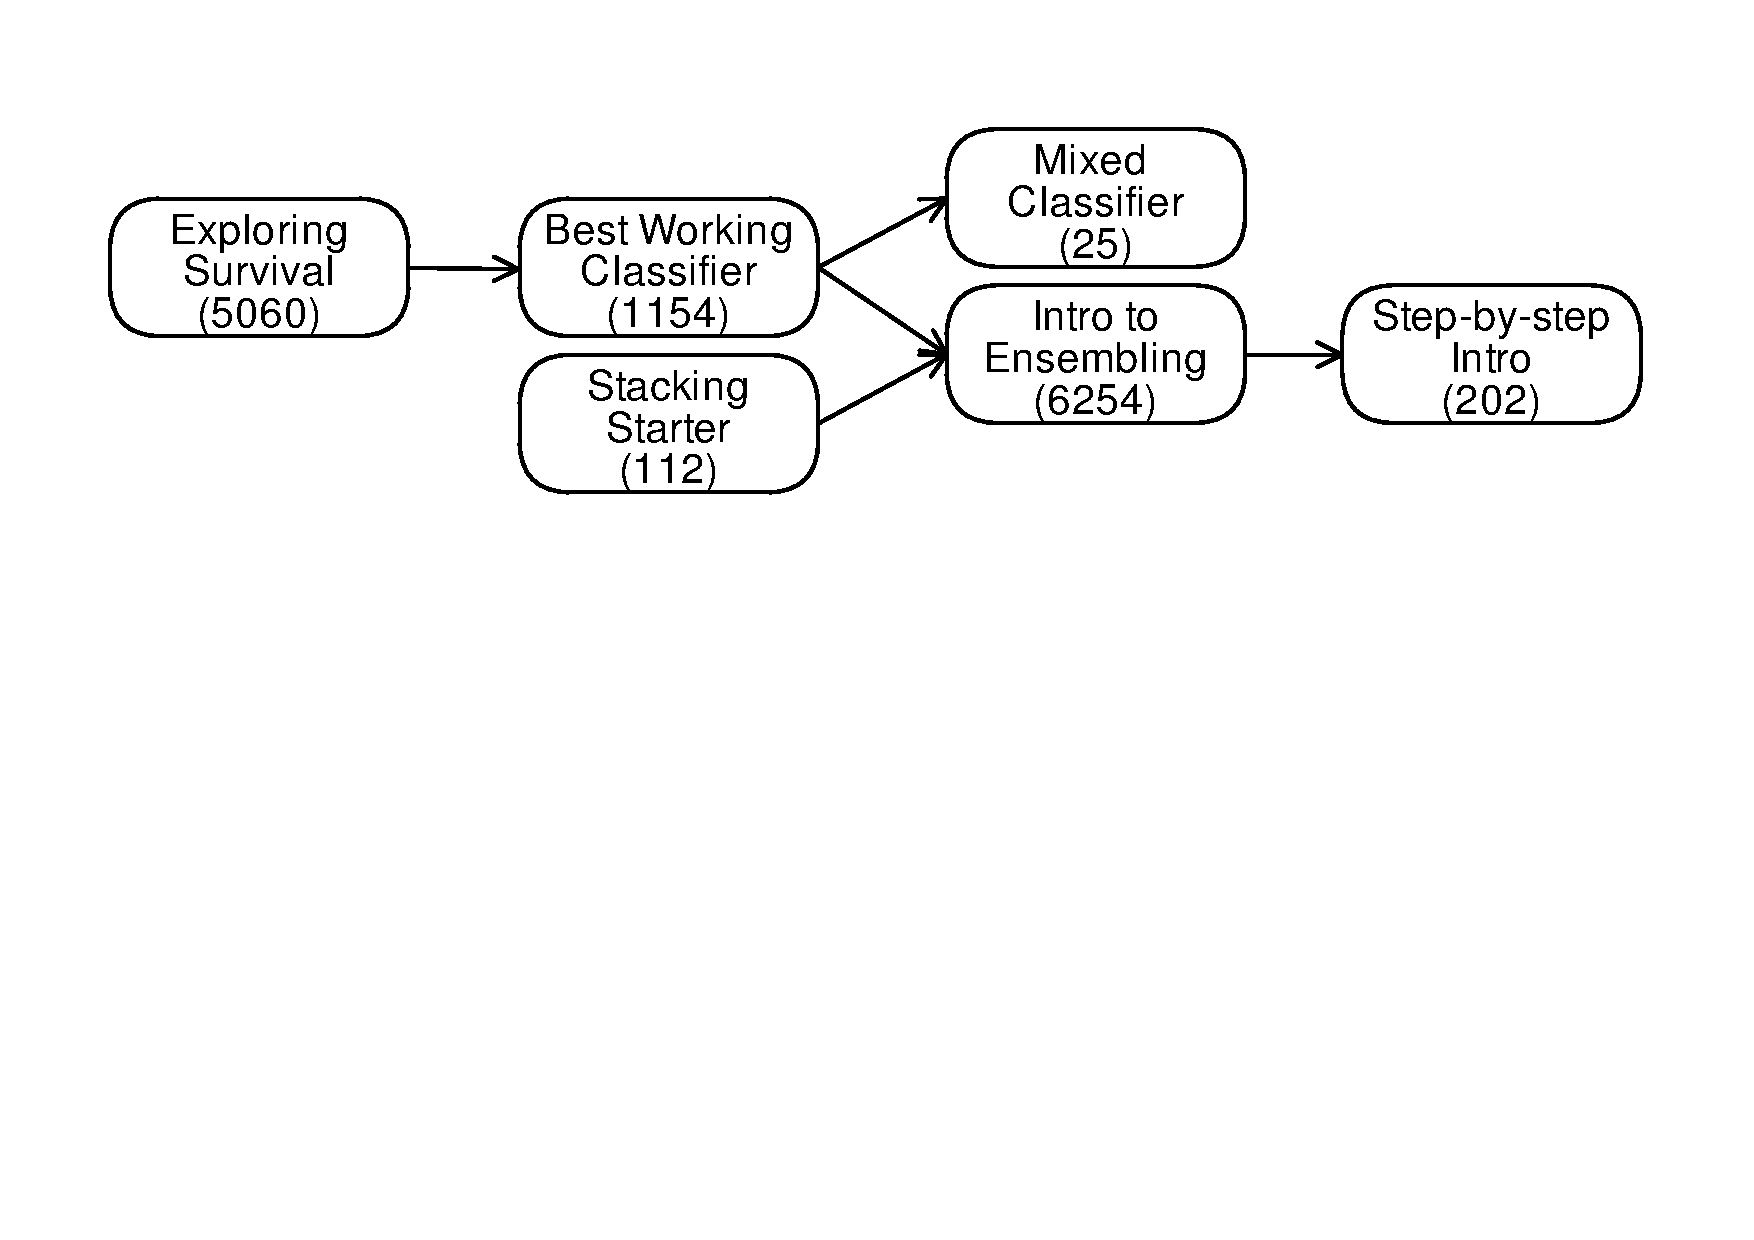
\includegraphics[width=\columnwidth]{../images/kaggle-titanic-scripts-graph}
\caption{The fork hierarchy of some of the popular kernels in Kaggle's Titanic competition}
\label{fig-titanic-script-hierarchy}
\end{figure}
For example, in the kernel \textbf{Best Working Classifier}, the author explicitly cites the kernel \textbf{Exploring Survival} as his/her inspiration.
The numbers show how many times other users copy a kernel into their workspace.
%TODO this number is pretty old, I should update it (or better yet do one figure from the competition that I'm using for the experiment (i.e., home credit)
The most popular kernels for the Titanic competition have been copied a total of 44,434 times.
This demonstrates that many of the executed workloads share exact or similar operations.
Since Kaggle is using isolated docker containers for executing user workloads, they cannot detect similar operations and re-execute the operations multiple times.
Moreover, while users can view and study publicly available kernels, they are not able to directly access the intermediate artifacts, such as any preprocessed dataset or machine learning model belonging to the existing kernels.
As a result, users must re-execute a kernel to generate the desired artifact.

\subsection{Experiment Database}
Experiment databases include data and meta-data of different data analytics and machine learning experiments executed over time \cite{miao2018provdb, vanschoren2014openml, schelter2017automatically, vartak2016m}.
They include different information about datasets, data processing pipeline components, machine learning models, execution of machine learning training algorithms, and quality of the models. 
Moreover, some experiment databases allow users to store some of the artifacts generated during the execution of a workload, such as raw datasets, intermediate datasets (resulting from applying data transformation operations), and machine learning models and their hyperparameters.
However, due to limited storage space, experiment databases cannot store every artifact.
 
Experiment databases can help in designing a better future workload.
For example, users can query the database to find the answer to the following questions: what type of data transformations and model training operations are executed on a dataset and what is the accuracy of the final models?
As a result, users can avoid executing data transformations or model training operations that do not result in high-quality models.
Moreover, experiment databases enable reproducibility and validation of results.
For example, users can query information about the environment and list of operations in a specific workload.
As a result, users can re-execute the workload and compare the results.